\documentclass[8pt]{beamer}

\setbeamertemplate{background canvas}[vertical shading][bottom=cyan!10,top=blue!10]

\usetheme{Warsaw}
\usefonttheme[onlysmall]{structurebold}

% pour le fichiers .pdf
\usepackage{graphicx}
\usepackage{color}
% pour les fichiers .png
% \usepackage{pgf,pgfarrows}
% \usepackage{pgf,pgfarrows}
\usepackage{amsmath,amssymb}
\usepackage{textcomp}
\usepackage{Math_Notations}
\usepackage{multitoc}
\usepackage{mdwtab}
\setbeamercovered{dynamic}
\DeclareMathOperator*{\argmin}{argmin}

\title[OpenTURNS Developer training]{OpenTURNS Developer training: first steps}
\author[OpenTURNS Consortium, 2019]
{
  Trainer : R\'egis LEBRUN\\
  Airbus \\
  regis.lebrun@airbus.com
}



\date[May 14-17th 2019]
{
  Developers training \\

  \begin{center}
    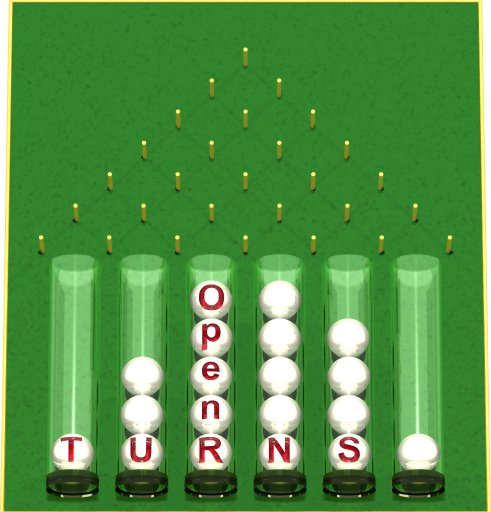
\includegraphics[height=2cm]{logoOT.jpg}
  \end{center}
}

\subject{OpenTURNS Developers Training}

\begin{document}

\frame{\titlepage}

% necessaire pour la table des matieres
\part{Main part}

% table des matieres
\begin{frame}
  \frametitle{OpenTURNS: first steps}
  \tableofcontents[part=1]
\end{frame}

\section{Navigation in the source code}

%%%%%%%%%%%%%%%%%%%%%%%%%%%%%%%%% 
% Navigation in the source code %
%%%%%%%%%%%%%%%%%%%%%%%%%%%%%%%%% 
\begin{frame}
  \frametitle{Navigation in the source code}
  \begin{block}{The Uniform distribution}
    \begin{itemize}
    \item Locate the class within the library source code;
    \item Follow its inheritance graph in order to explore the Bridge pattern;
    \item Locate the associated regression test;
    \item Execute the test;
    \item Locate its SWIG interface file and its associated Python module;
    \item Execute the associated python test.
    \end{itemize}
  \end{block}
\end{frame}


\section{Library development}

%%%%%%%%%%%%%%%%%% 
% Global picture %
%%%%%%%%%%%%%%%%%% 
\begin{frame}
  \frametitle{Library development 1/9}
  \begin{block}{Projects}
    \begin{enumerate}
    \item~(*) \alert{\ttfamily InverseDistanceWeightingInterpolation} as a specialization of \alert{\ttfamily EvaluationImplementation} (see {\ttfamily lib/src/Base/Func}). Given a set of data $(x_i, y_i)_{i=1,\dots,N}$ in $\R^n\times\R^p$, the IDW interpolation is defined by:
      \begin{align}
        \forall x\in\R^n, u(x)=\left\{\begin{array}{ll}
                                        \dfrac{\sum_{i=1}^Nw_i(x)y_i}{\sum_{i=1}^Nw_i(x)} & \mbox{ if } \forall i, d(x, x_i) > 0\\
                                        y_i & \mbox{ if } \exists i, d(x, x_i)=0
                                      \end{array}
                                              \right.
      \end{align}
      where $w_i(x)=\dfrac{1}{d(x, x_i)^p}$ and $p>0$ a given smoothness parameter.

      The distance $d$ can be the Euclidean distance, the 1-norm or the sup norm.
    \item~(**) \alert{\ttfamily DiscreteIntegralCompound} as a specialization of \alert{\ttfamily DiscreteDistribution} (see {\ttfamily lib/src/Uncertainty/Distribution}). Given the discrete distribution of a random variable $N$ and the common discrete distribution of a sequence of iid integral valued random variables $(X_i)$, compute the distribution of the integral valued discrete random variable $Y$ defined by:
      \begin{align}
        Y = \sum_{i=1}^N X_i
      \end{align}
    \end{enumerate}
  \end{block}
\end{frame}

\begin{frame}
  \frametitle{Library development 2/9}
  \begin{block}{Projects}
    \begin{enumerate}
    \item[] Its generating function $\phi_Y(z)=\Esp{z^Y}$ is given by:
      \begin{align}
        \forall z\in\C, \phi_Y(z)=\phi_N(\phi_X(z))
      \end{align}
      and thanks to Poisson's summation formula for discrete distributions, we have for $0<r<1$ and $m\in\N^*$:
      \begin{eqnarray}\label{pnApprox}
        \forall n\in\{0,\dots, m-1\}, p_Y(n) = \displaystyle \frac{1}{mr^n} \sum_{k=0}^{m-1} \phi_Y\left(re^{\frac{2i\pi k}{m}}\right) e^{-\frac{2i\pi kn}{m}} - e_d
      \end{eqnarray}
      where $0\leq e_d\leq r^m$ is the approximation error. For a given $\epsilon>0$ and $m\in\N^*$, set $r=\sqrt[m]{\epsilon}$ and compute the FFT $(\omega_0,\dots,\omega_{m-1})$ of the complex vector $(\phi_Y\left(re^{\frac{2i\pi k}{m}}\right), \dots, \phi_Y\left(re^{\frac{2i\pi k}{m}}\right))$. Then, the distribution is equal to the {\ttfamily UserDefined} distribution with locations $\{0,\dots,m-1\}$ and probabilities $\left(p_i=\dfrac{\mathfrak{R}(\omega_i)}{mr^i}\right)_{i=0,\dots,m-1}$.
    \end{enumerate}
  \end{block}
\end{frame}

\begin{frame}
  \frametitle{Library development 3/9}
  \begin{block}{Projects}
    \begin{enumerate}
      \setcounter{enumi}{2}
    \item~(*) \alert{\ttfamily ClenshawCurtis} integration algorithm as a specialization of \alert{\ttfamily IntegrationAlgorithmImplementation} (see {\ttfamily lib/src/Base/Algo}). This integration algorithm allows to compute integrals of the form:
      \begin{align*}
        I(f)=&\int_a^bf(t)\,dt\\
        =&\dfrac{b-a}{2}\int_{-1}^1f\left(a+\dfrac{b-a}{2}(1+x)\right)\,dx\\
           \simeq& \dfrac{b-a}{2}\sum_{k=0}^nw_kf(a+\dfrac{b-a}{2}(1+x_k))
      \end{align*}
      where $x_k=\cos\theta_k$, $\theta_k=\dfrac{k\pi}{n}$ and $w_k$ is given by:
      \begin{align}
        w_k=\dfrac{c_k}{n}\left(1-\sum_{j=1}{\lfloor n/2\rfloor}\dfrac{b_j}{4j^2-1}\cos\left(2j\theta_k\right)\right)
      \end{align}
    \end{enumerate}
  \end{block}
\end{frame}

\begin{frame}
  \frametitle{Library development 4/9}
  \begin{block}{Projects}
    \begin{enumerate}
      \setcounter{enumi}{3}
      \item[] where the coefficients $b_j$ and $c_k$ are given by:
      \begin{align}
        b_j=\left\{\begin{array}{ll}
                     1 & j = n/2 \\
                     2 & j < n/2
                     \end{array}\right.\quad c_k=\left\{\begin{array}{ll}
                     1 & k = 0[n] \\
                     2 & k\neq 0[n]
                     \end{array}\right.
      \end{align}
      for $k=0,\dots,n$. An efficient FFT-based implementation of the computation of the weights and nodes is given in {\ttfamily fclencurt.m}, another one (**) in {\ttfamily 1311.0445.pdf}.
    \item~(*) \alert{\ttfamily Fejer1} integration algorithm as a specialization of  \alert{\ttfamily IntegrationAlgorithmImplementation} (see {\ttfamily lib/src/Base/Algo}). This integration algorithm is based on the nodes $x_k=\cos\theta_{k+1/2}$ and weights:
      \begin{align}
        w_k^{f1}=\dfrac{2}{n}\left(1-2\sum_{j=1}^{\lfloor n/2\rfloor}\dfrac{1}{4j^2-1}\cos\left(j\theta_{2k+1}\right)\right)
      \end{align}
      for $k=0,\dots,\alert{n-1}$. There also exist fast implementations based on FFT or modified moments, see the references for Clenshaw Curtis.
    \end{enumerate}
  \end{block}
\end{frame}

\begin{frame}
  \frametitle{Library development 5/9}
  \begin{block}{Projects}
    \begin{enumerate}
      \setcounter{enumi}{4}
    \item~(*) \alert{\ttfamily Fejer2} integration algorithm as a specialization of  \alert{\ttfamily IntegrationAlgorithmImplementation} (see {\ttfamily lib/src/Base/Algo}). This integration algorithm is based on the nodes $x_k=\cos\theta_k$ and weights:
      \begin{align}
        w_k^{f2}=\dfrac{4}{n}\sin\theta_k\sum_{j=1}{\lfloor n/2\rfloor}\dfrac{\sin\left((2j-1)\theta_k\right)}{2j-1}
      \end{align}
      for $k=0,\dots,n$. There also exist fast implementations based on FFT or modified moments, see the references for Clenshaw Curtis.
    \item~(**) \alert{\ttfamily ClenshawCurtisProductExperiment} as a specialization of {\ttfamily WeightedExperiment}: same algorithm as for {\ttfamily ClenshawCurtis} but with adaptation to any weight function.
    \item~(*) \alert{\ttfamily MarshallOlkinCopula} as a specialization of {\ttfamily CopulaImplementation} (see {\ttfamily lib/src/Uncertainty/Distribution}). This copula is defined by:
      \begin{equation}
        \forall (u,v)\in[0,1]^2, C(u, v)=\left\{
          \begin{array}{ll}
            u^{1-\alpha}v & \mbox{ for }u^\alpha\geq v^\beta \\
            uv^{1-\beta} & \mbox{ for }u^\alpha< v^\beta
          \end{array}{ll}
        \right.
      \end{equation}
      where $0<\alpha, \beta<1$.
    \end{enumerate}
  \end{block}
\end{frame}

\begin{frame}
  \frametitle{Library development 6/9}
  \begin{block}{Projects}
    \begin{enumerate}
      \setcounter{enumi}{7}
    \item~(*) \alert{\ttfamily GumbelCopula} as a specialization of {\ttfamily ExtremeValueCopula} (see {\ttfamily lib/src/Uncertainty/Distribution}). This copula already exists, but not as an extreme value copula. It is defined by its Pickand function:
      \begin{align}
        \forall t\in[0,1], A(t)=\left[t^\theta+(1-t)^\theta\right]^{1/\theta}
      \end{align}
      where $\theta\geq 1$. 
    \item~(*) \alert{\ttfamily GalambosCopula} as a specialization of {\ttfamily ExtremeValueCopula} (see {\ttfamily lib/src/Uncertainty/Distribution}). This copula is defined by its Pickand function:
      \begin{align}
        \forall t\in[0,1], A(t)=1-\left[t^{-\theta}+(1-t)^{-\theta}\right]^{-1/\theta}
      \end{align}
      where $\theta\geq 0$.
    \item~(*) \alert{\ttfamily TawnCopula} as a specialization of {\ttfamily ExtremeValueCopula} (see {\ttfamily lib/src/Uncertainty/Distribution}). This copula is defined by its Pickand function:
      \begin{align}
        \forall t\in[0,1], A(t)=(1-\psi_1)(1-t)+(1-\psi_2)t+\left[\left\{\psi_1t\right\}^{1/\theta}+\left\{\psi_2(1-t)\right\}^{1/\theta}\right]^\theta
      \end{align}
      where $0<\theta\leq 1$ and $0\leq\psi_1,\psi_2\leq 1$.
    \end{enumerate}
  \end{block}
\end{frame}

\begin{frame}
  \frametitle{Library development 7/9}
  \begin{block}{Projects}
    \begin{enumerate}
      \setcounter{enumi}{10}
    \item~(*) \alert{\ttfamily JoeCopula} as a specialization of {\ttfamily ExtremeValueCopula} (see {\ttfamily lib/src/Uncertainty/Distribution}). This copula is defined by its Pickand function:
      \begin{align}
        \forall t\in[0,1], A(t)=1-\left[\left\{\psi_1(1-t)\right\}^{-1/\theta}+\left\{\psi_2t\right\}^{-1/\theta}\right]^{-\theta}
      \end{align}
      where $\theta>0$ and $0\leq\psi_1,\psi_2\leq 1$.
    \item~(**) \alert{\ttfamily ArchiMaxCopula} as a specialization of {\ttfamily CopulaImplementation} (see {\ttfamily lib/src/Uncertainty/Distribution}). Given an Archimedean copula with generator $\psi$ and an extreme value copula with Pickand function $A$, an archimax copula $C$ is defined by:
      \begin{align}
        \forall (u,v)\in[0,1]^2, C(u,v)=\psi^{-1}\left(\min\left(\psi(0), [\psi(u)+\psi(v)]A\left(\dfrac{\psi(u)}{\psi(u)+\psi(v)}\right)\right)\right)
      \end{align}
      It becomes (***) if one wants to implement an efficient sampling algorithm.
    \end{enumerate}
  \end{block}
\end{frame}

\begin{frame}
  \frametitle{Library development 8/9}
  \begin{block}{Projects}
    \begin{enumerate}
      \setcounter{enumi}{12}
    \item~(*) \alert{\ttfamily SquaredNormal} as a specialization of {\ttfamily ContinuousDistribution} (see {\ttfamily lib/src/Uncertainty/Distribution}). If $X$ is distributed according to the $\cn(\mu,\sigma)$ distribution, $Y=X^2$ is distributed according to the squared normal distribution with parameters $\mu$ and $\sigma>0$. This distribution has already been implemented in Python, see {\ttfamily SquaredNormal.py}.
    \item~(**) \alert{\ttfamily ConditionalEventDistribution} as a specialization of {\ttfamily ContinuousDistribution} (see {\ttfamily lib/src/Uncertainty/Distribution}). Given the joint distribution of an $(m+n)$ dimensional random vector $(X,Y)$ and an $m$ dimensional interval $I$ such that $\Prob{X\in I}>0$, it is the distribution of $Y$ knowing that $X\in I$. This distribution has already been implemented in Python, see {\ttfamily ConditionalEventDistribution.py}. It becomes (***) if one wants to implement an efficient simplification mechanism.
    \item~(***) Extend archimedian copulas from 2-d to $n$-d. Given a 2-d Archimedean copula with generator $\psi$, implement its $n$-d counterpart using:
      \begin{align}
        \forall (u_1,\dots,u_n)\in[0,1]^n, C(u_1,\dots,u_n)=\psi^{-1}\left(\psi(u_1)+\dots+\psi(u_n)\right)
      \end{align}
      The main difficulties are the architecture of this extension and the implementation of an efficient sampling algorithm.
    \end{enumerate}
  \end{block}
\end{frame}

\begin{frame}
  \frametitle{Library development 9/9}
  \begin{block}{Projects}
    \begin{enumerate}
      \setcounter{enumi}{15}
    \item~(**) \alert{\ttfamily BlockComposedDistribution} as a specialization of {\ttfamily DistributionImplementation} (see {\ttfamily lib/src/Uncertainty/Distribution}). Given a collection of distributions $D_1,\dots,D_n$ of dimensions $d_1,\dots,d_n$, it is the distribution of the random vector $(X_1,\dots,X_n)$ of dimension $d_1+\dots+d_n$ where $X_i$ is distributed as $D_i$ and $X_1,\dots,X_n$ are independent.

      It becomes (****) if one wants to propagate this new distribution in every places it could go within the library.
    \item~(*) Extend \alert{\ttfamily SolverImplementation} and \alert{\ttfamily Solver} to the resolution of systems of nonlinear equations and provide a generic implementation using the \alert{\ttfamily LeastSquaresProblem} class. The solutions $x^*$ of a nonlinear system of equations $f_1(x)=0,\dots,f_n(x)=0$ where $x=(x_1,\dots,x_n)$, if they exist, have to be found in the set of solutions of the following least-squares problem:
      \begin{align}
        x^*=\arg\min \sum_{j=1}^n f_j^2(x)
      \end{align}
      for which many solvers are available in OpenTURNS.
    \end{enumerate}
  \end{block}
\end{frame}

\section{Module development}

\begin{frame}
  \frametitle{Module development 1/2}
  \begin{block}{Projects}
    \begin{enumerate}
      \setcounter{enumi}{17}
    \item~(*) or (**) \alert{\ttfamily CloudMesher}: mesh generation over a cloud of points using kernel mixture, pca, rotation, then levelset mesher on an interval
    \item~(*) \alert{\ttfamily UniformSphereRandomVector} as a specialization of {\ttfamily RandomVectorImplementation} (see {\ttfamily lib/src/Uncertainty/Model}). This random vector is distributed uniformly on the sphere of center $c\in\R^n$ and radius $r>0$. The sampling is done using the fact that $Y/\|Y\|$ is uniformly distributed over $\cs_{n-1}$, the unit sphere in $\R^n$, if $Y$ is an $n$ dimensional random vector with independent $\cn(0,1)$ components.
    \item~(*) \alert{\ttfamily UniformBallRandomVector} as a specialization of {\ttfamily RandomVectorImplementation} (see {\ttfamily lib/src/Uncertainty/Model}). This random vector is distributed uniformly on the ball of center $c\in\R^n$ and radius $r>0$. The sampling is done using the fact that $Y/\sqrt{\|Y\|^2+Z}$ is uniformly distributed over $\cb_{n-1}$, the unit ball in $\R^n$, if $Y$ is an $n$ dimensional random vector with independent $\cn(0,1)$ components, and $Z$ is $\ce(1)$ independent from $Y$.
    \item~(*) \alert{\ttfamily UniformSimplexRandomVector} as a specialization of {\ttfamily RandomVectorImplementation} (see {\ttfamily lib/src/Uncertainty/Model}). This random vector is distributed uniformly in the simplex given by $n+1$ points in $\R^n$. The sampling is done using the fact that $Y$ is uniformly distributed over the standard simplex in $\R^n$ if it follows the Dirichlet distribution with parameter $(\theta_1=1,\dots,\theta_n=1)$.
    \end{enumerate}
  \end{block}
\end{frame}

\begin{frame}
  \frametitle{Module development 2/2}
  \begin{block}{Projects}
    \begin{enumerate}
      \setcounter{enumi}{21}
    \item~(**) \alert{\ttfamily SmoliakExperiment} as a specialization of {\ttfamily WeightedExperiment} (see {\ttfamily lib/src/Uncertainty/Algorithm/WeightedExperiment}). This design of experiment is obtained by interfacing the smolpack C library. A possible name for the module is \alert{OTSmolpack}.
    \item~(**) \alert{\ttfamily CubaIntegration} as a specialization of {\ttfamily IntegrationAlgorithmImplementation} (see {\ttfamily lib/src/Base/algo}). This algorithm is obtained by interfacing the cuba C library. A possible name for the module is \alert{OTCuba}.
    \item~(**) \alert{\ttfamily HIntLibIntegration} as a specialization of {\ttfamily IntegrationAlgorithmImplementation} (see {\ttfamily lib/src/Base/algo}). This algorithm is obtained by interfacing the HIntLib C++ library, see \alert{https://github.com/JohannesBuchner/HIntLib}. A possible name for the module is \alert{OTHIntLib}.
    \end{enumerate}
  \end{block}
\end{frame}
\end{document}
